\chapter[Généralisation aux surfaces de topologie quelconque]{Généralisation aux surfaces régulières par~morceaux de topologie quelconque}
\label{chap:multi_patch}

\section{Construction des nouvelles faces}

objectif : définir la paramétrisation des nouvelles surfaces (et les limites du domaine paramétrique pour les faces \brep\ reposant sur celles-ci)

\subsection{Arêtes convexes}
paramétrisation approchée des courbes d'intersection (choix du paramètre : abscisse curviligne, paramètre de Hohmeyer (cf. \autoref{sec:calcul_intersections}), \eng{least-square fitting} (ajustement de courbe par la méthode des moindres carrés) d'une série de Chebyshev univariée), portion de \eng{canal surface} approchée 

\subsection{Sommets convexes}
deux variantes :

\subsubsection{Une face polygonale}
$(u,v) \equiv$ coordonnées sphériques\\
+ : 1 seule face, spectre Chebyshev étroit/compact


\subsubsection{Plusieurs faces rectangulaires}
polygone sphérique découpé en quadrilatères \cite{hahn1989}\\
+ : domaine paramétrique non restreint


\section{Résolution des intersections entre faces}
\subsection{État de l'art}
état de l'art méthodes d'intersection de surfaces paramétriques :
review complète $\to$ \cite{patrikalakis2009}\\
subdivision \cite{houghton1985}, implicitisation approchée \cite{dokken2001}, suivi (marching) \cite{barnhill1990}, Hohmeyer \cite{hohmeyer1992} (critère de détection de boucles sur les enveloppes de normales, paramétrisation monotone et tracé des branches d'intersection)


\subsection{Approche retenue}
\label{sec:calcul_intersections}
adaptation de l'approche de Hohmeyer \cite{hohmeyer1992} (full Chebyshev / Chebyshev-Bernstein)
\begin{itemize}
	\item changement de base \cite{rababah2003}
	\item volumes englobants convexes : oriented bounding box \cite{fournier1994} (détail en \autoref{app:obb}) / enveloppe convexe (comparer complexité, volumes)
	\item subdivision : changement de variable (détail en \autoref{app:cdv_cheb}) / algorithme de Casteljau (ref?) 
	\item test de séparation : théorème de séparation des convexes \cite{eberly2002} / optimisation linéaire \cite{seidel1991}
	\item traitement des intersections tangentielles
\end{itemize}



\section{Validation de la méthode}

\subsection{Propagation suivant un champ de vitesse continu}
sphère/cube dans un écoulement tourbillonnaire incompressible analytique de période temporelle $2T$\\
\begin{equation}
	\vrm{u}(x,y,z,t) = 
	%\cos \left( \frac{\pi t}{T} \right)
	\cos( \pi t/T )
	\colvec{
	\sin^2(\pi x) \left[ \sin(2\pi z) - \sin(2\pi y)\right] \\
\sin^2(\pi y) \left[ \sin(2\pi x) - \sin(2\pi z)\right] \\
\sin^2(\pi z) \left[ \sin(2\pi y) - \sin(2\pi x)\right]
	}.
\end{equation}
%\begin{figure}
%	\centering
%	\newdimen\imwid
\imwid=0.49\linewidth
\newdimen\rad
\rad=0.12\imwid
\newdimen\ticklen
\ticklen=3pt
\newdimen\imyshift
\imyshift=\rad
\begin{tikzpicture}[%
	img/.style={inner sep=0pt},%
	txt/.style={font=\small, inner sep=2pt},%
	axe/.style={line width=0.5pt}%
	]%
	%
	\node[anchor=south east, yshift=-\imyshift] (im1) {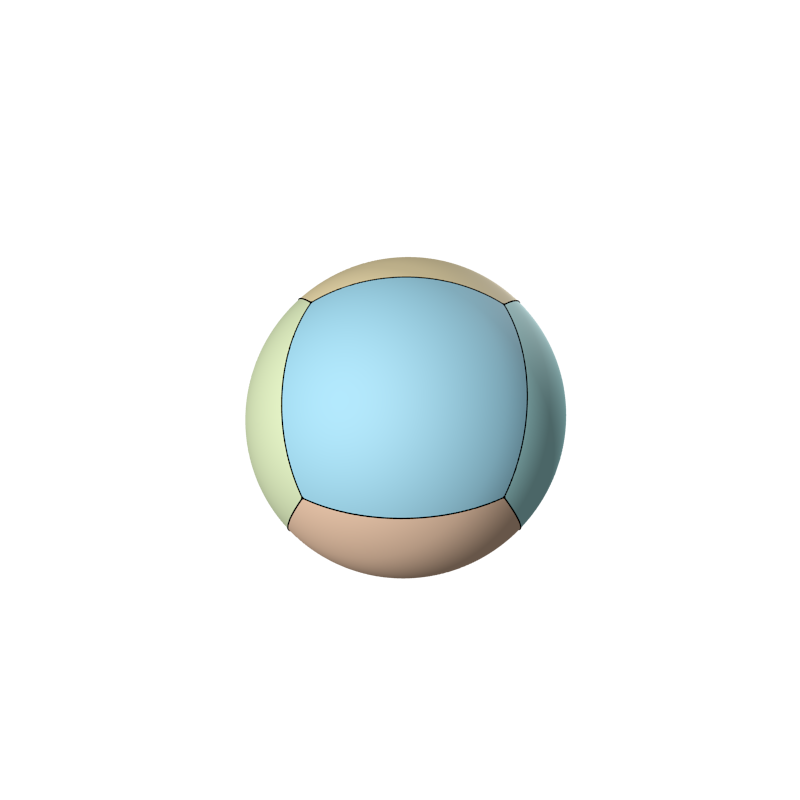
\includegraphics[width=\imwid]{figures/snap_001}};
	\node[anchor=south west, yshift=-\imyshift] (im2) {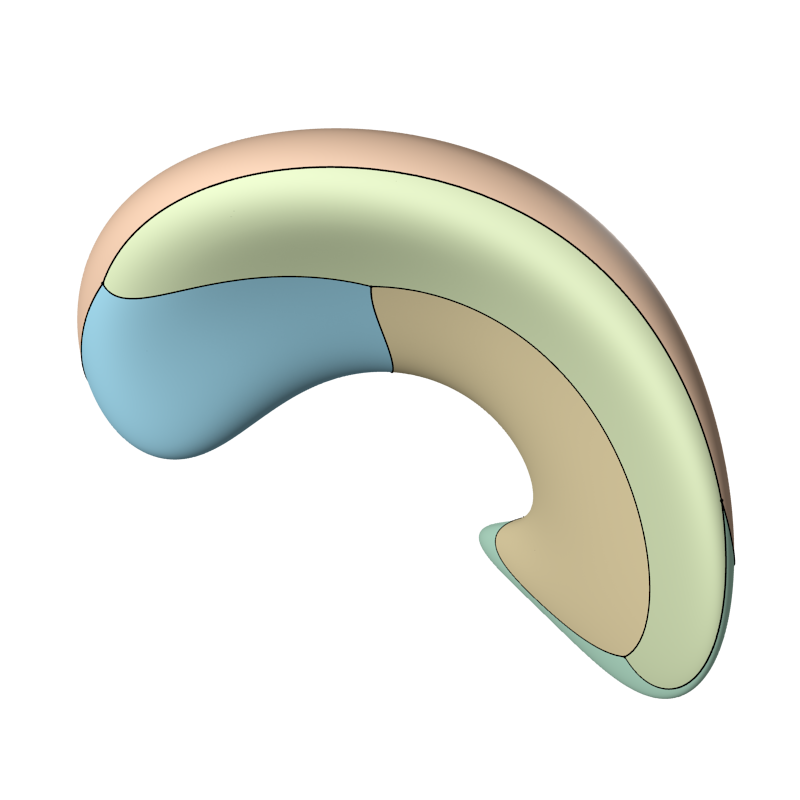
\includegraphics[width=\imwid]{figures/snap_002}};
	\node[anchor=north west, yshift=-\imyshift] (im3) {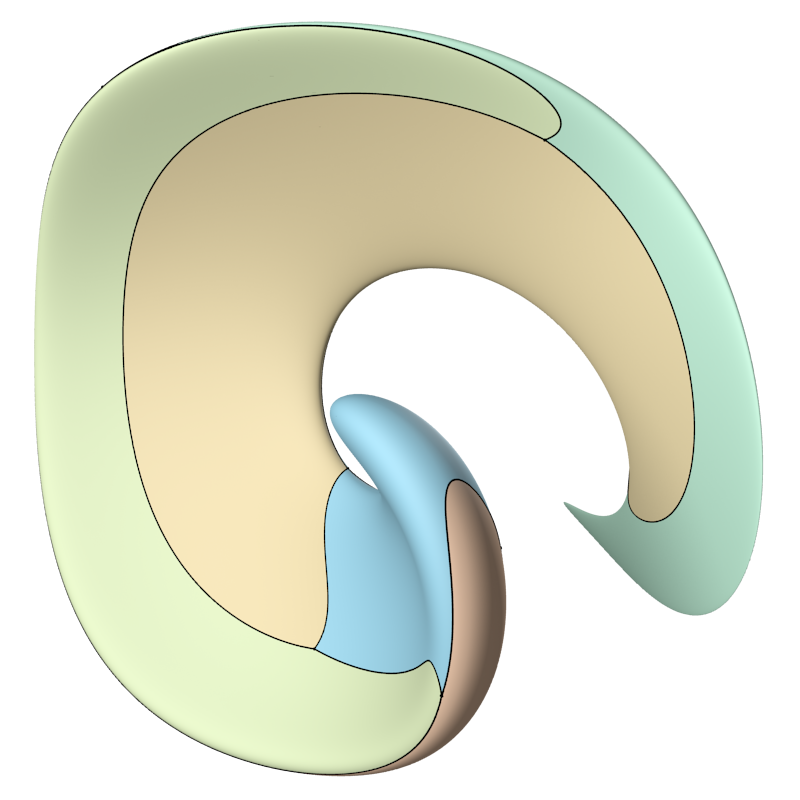
\includegraphics[width=\imwid]{figures/snap_003}};
	\node[anchor=north east, yshift=-\imyshift] (im4) {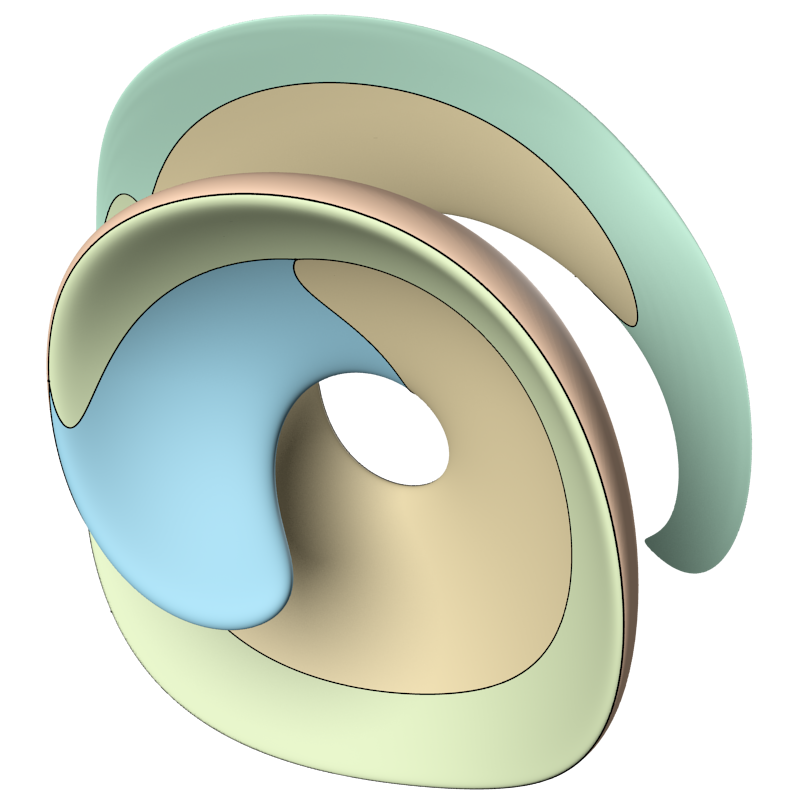
\includegraphics[width=\imwid]{figures/snap_005}};
    %
    \draw[-latex', axe] (0,0) + (135:\rad) arc(135:-180:\rad) node[txt, left, xshift=-1pt] {$t/T$};
    \draw[axe, dash pattern=on 2pt off 2pt] (0,0) + (135:\rad) arc(135:165:\rad);
    \foreach \a in {135,45,-45,-135}
    {%
    	\draw[axe] (\a:\rad-0.5\ticklen)--(\a:\rad+0.5\ticklen);
    }%
    \node[anchor=south east, txt] at (135:\rad) {$0$} ;
    \node[anchor=south west, txt] at (45:\rad) {$1/8$} ;
    \node[anchor=north west, txt] at (-45:\rad) {$1/4$} ;
    \node[anchor=north east, txt] at (-135:\rad) {$1/2$} ;
\end{tikzpicture}
%	\caption{Modèle \brep\ à différents instants de la déformation ($T=4$).}
%	\label{fig:snapshots_vortex}
%\end{figure}

\begin{figure}
	\centering
	\newdimen\imwid
\imwid=0.49\linewidth
\newdimen\imypos
\imypos=1.1\imwid
\def\imangle{0}
\begin{tikzpicture}[%
	img/.style={inner sep=0pt},%
	txt/.style={font=\normalsize, inner sep=2pt, anchor=south west}%
	]%
	%
	\node (im1) at (0,0) {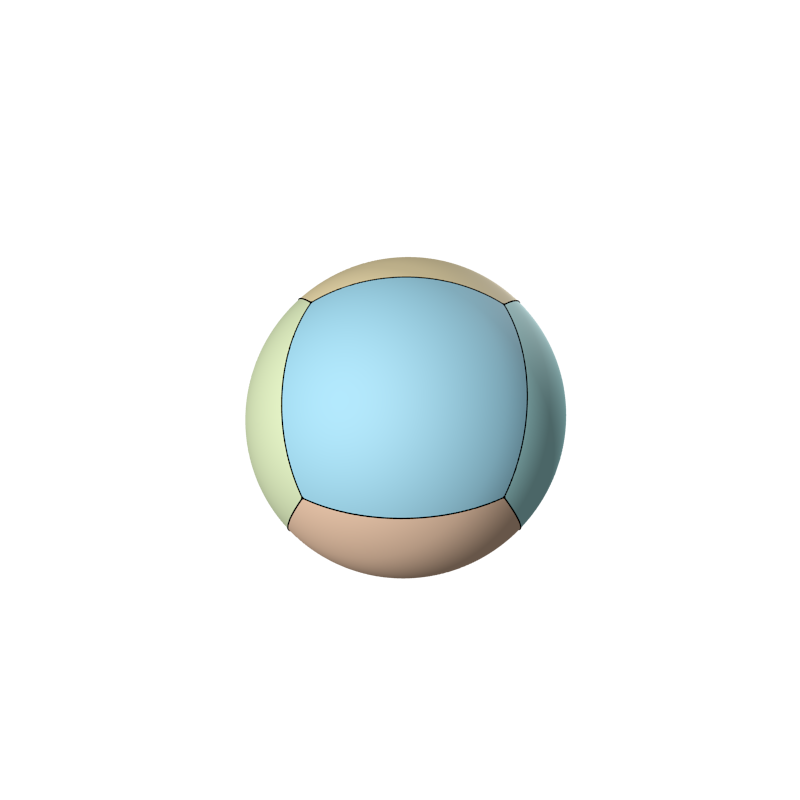
\includegraphics[width=\imwid, angle=\imangle]{figures/snap_001}};
	\node (im2) at (\imwid,0) {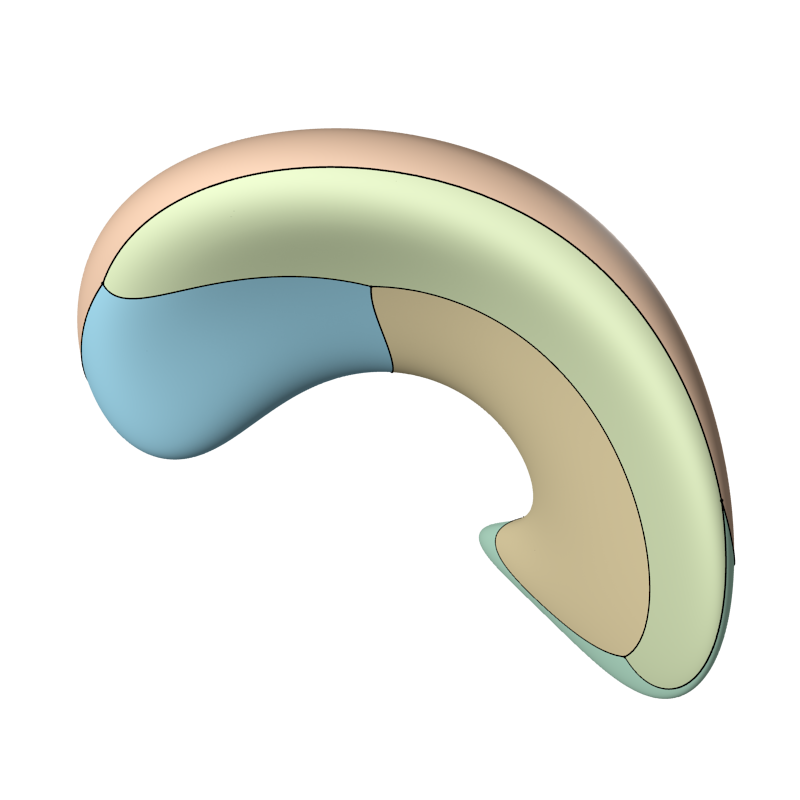
\includegraphics[width=\imwid, angle=\imangle]{figures/snap_002}};
	\node (im3) at (0,-\imypos) {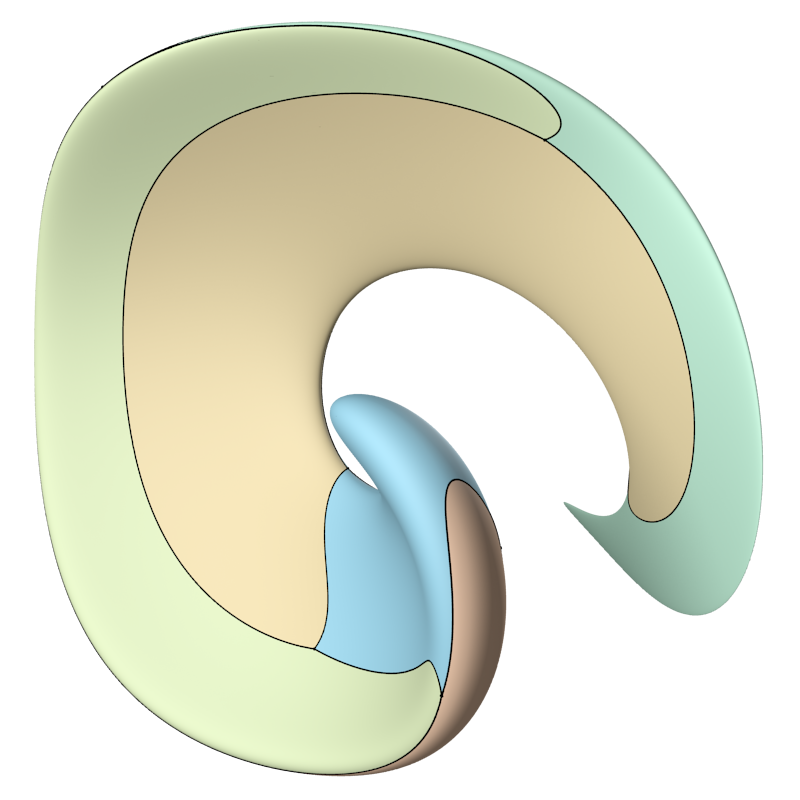
\includegraphics[width=\imwid, angle=\imangle]{figures/snap_003}};
	\node (im4) at (\imwid,-\imypos) {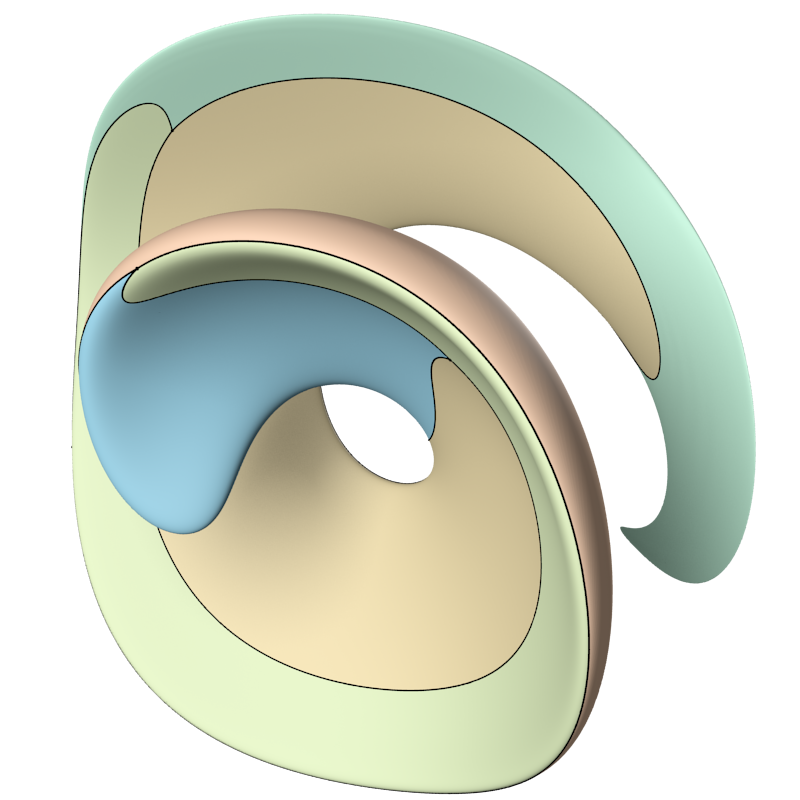
\includegraphics[width=\imwid, angle=\imangle]{figures/snap_004}};
	\node (im5) at (0,-2\imypos) {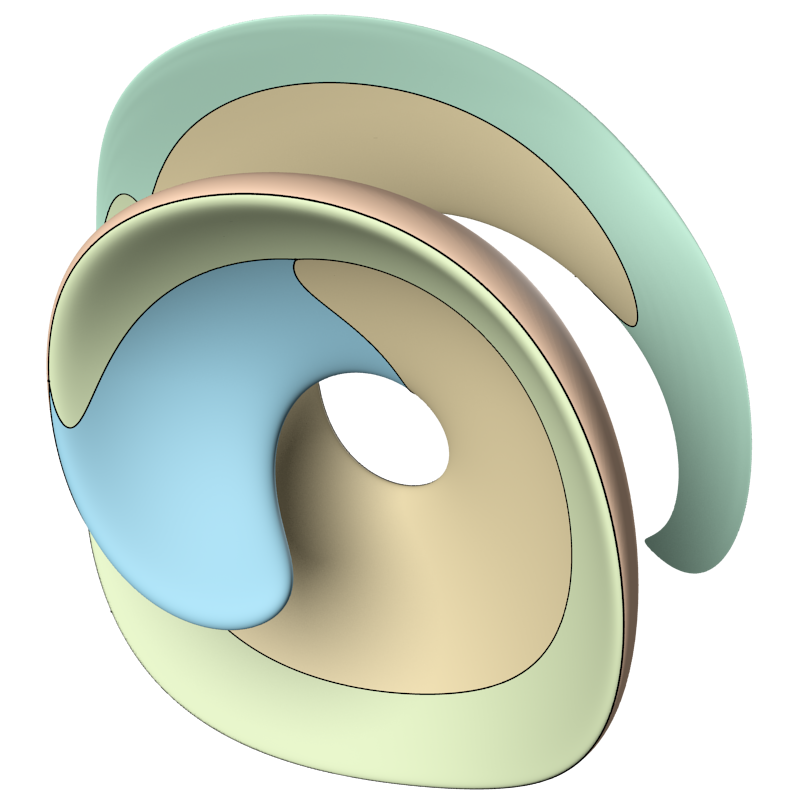
\includegraphics[width=\imwid, angle=\imangle]{figures/snap_005}};
	\node (im6) at (\imwid,-2\imypos) {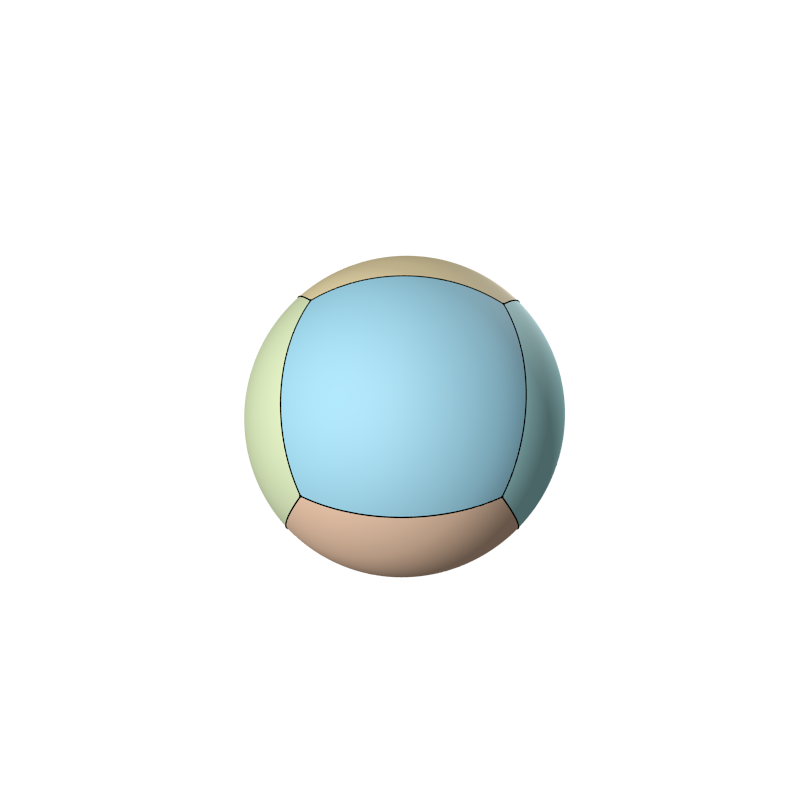
\includegraphics[width=\imwid, angle=\imangle]{figures/snap_006}};
	%
	\node[txt] at (im1.south west) {$t=0$} ;
    \node[txt] at (im2.south west) {$t=T/8$} ;
    \node[txt] at (im3.south west) {$t=T/4$} ;
    \node[txt] at (im4.south west) {$t=3T/8$} ;
    \node[txt] at (im5.south west) {$t=T/2$} ;
    \node[txt] at (im6.south west) {$t=T$} ;
\end{tikzpicture}
	\caption{Modèle \brep\ à différents instants de la déformation ($T=4$).}
	\label{fig:snapshots_vortex}
\end{figure}
paramétrisation : cube projeté sur sphère\\
calcul de volume avec quadrature de Clenshaw-Curtis (exact, l'intégrande est polynomiale) (étanchéité (continuité $G^0$ partout) garantie car les marqueurs de bord coïncident tout au long de la déformation)\\
convergence de l'erreur d'approximation sur la position, l'aire et le volume à $t = 0$ et $t = T$ pour différents niveaux de discrétisations spatiale et temporelle\\

%%%%%%%%%%%%%%%
% figures erreur vs dof
%%%%%%%%%%%%%%
\def\axw{0.48\textwidth}
\def\axh{0.39\textwidth}
\def\xlabl{$N$}%{$\mathrm{dof}$}
\def\ylabl{Erreur}
\def\xsep{2pt}
%%%%%%%%%%%%%%
\plotvortexerrorc{position}{la~}{pos}{maximale}
%%%%%%%%%%%%%%
\plotvortexerrorc{aire}{l'}{air}{relative}
%%%%%%%%%%%%%%
\plotvortexerrorc{volume}{le~}{vol}{relative}
%%%%%%%%%%%%%%
%%%%%%%%%%%%%%%
%\def\xlabl{$N$}%\mathrm{dof}^{0.4}$}
%%%%%%%%%%%%%%%
%\plotvortexerrorb{position}{la~}{pos}{maximale}
%%%%%%%%%%%%%%%
%\plotvortexerrorb{aire}{l'}{air}{relative}
%%%%%%%%%%%%%%%
%\plotvortexerrorb{volume}{le~}{vol}{relative}
%%%%%%%%%%%%%%%
%%%%%%%%%%%%%%%

+ convergence de la variation de volume au cours de la déformation\\
%https://tex.stackexchange.com/questions/23993/use-first-row-of-a-table-as-legend-entry-in-pgfplot-graph
%\begin{figure}
%  \centering
%  \begin{tikzpicture}%
%  \begin{semilogyaxis}[%
%    axis lines*=left,%
%    width=9cm, height=7cm,%
%    xmin = 0.0, xmax = 1.0,%
%    %ymin = 1e-16, ymax = 1e1,%
%    %ytickten = {-15,-10,-5,0},%
%    ymin = 1e-15, ymax = 1e0,%
%    ytickten = {-15,-10,-5,0},%
%    xtick distance=.25,
%    grid=major,%
%    xlabel={$t/T$},%
%    ylabel={$\frac{\left|V - V_0\right|}{V_0}$},%
%    %legend style={font=\small, at={(0.5,0.0)}, anchor=south, yshift=4pt},%
%    legend style={font=\small, at={(1.025,1.0)}, anchor=north west},%
%    no marks, each nth point=1]%
%    \pgfplotstableread{figures/data/vortex_erreur_volume_vs_time_0.001_bak.dat}   {\datatable}
%    \pgfplotstablegetcolsof{\datatable}
%    \pgfmathtruncatemacro\numberofcols{\pgfplotsretval-1}
%    \pgfplotsinvokeforeach{2,...,\numberofcols}{
%      \pgfplotstablegetcolumnnamebyindex{#1}\of{\datatable}\to{\colname}
%      \addplot+ table [y index=#1] from \datatable;%
%  	  \addlegendentryexpanded{$\mathrm{dof} = \colname$}
%    }%
%  \end{semilogyaxis}%
%  \end{tikzpicture}%
%  \caption{Évolution de l'erreur relative en volume au cours du temps, pour différents niveaux de discrétisation spatiale. Le schéma de Runge-Kutta explicite à l'ordre 4 est utilisé pour l'intégration temporelle, avec un pas de temps $\Delta t = 0.001$.}
%\end{figure}


\begin{figure}
  \centering
  \begin{tikzpicture}%
  \begin{semilogyaxis}[%
    axis lines*=left,%
    width=9cm, height=7cm,%
    xmin = 0.0, xmax = 1.0,%
    %ymin = 1e-16, ymax = 1e1,%
    %ytickten = {-15,-10,-5,0},%
    ymin = 1e-16, ymax = 1e0,%
    ytickten = {-16,-12,-8,-4,0},%
    xtick distance=.25,
    grid=major,%
    xlabel={$t/T$},%
    ylabel={$\frac{\left|V - V_0\right|}{V_0}$},%
    %legend style={font=\small, at={(0.5,0.0)}, anchor=south, yshift=4pt},%
    %legend style={font=\small, at={(1.025,1.0)}, anchor=north west},%
    legend style={font=\small, at={(0.5,0.033)}, anchor=south},%
    no marks, each nth point=1]%
    \pgfplotstableread{figures/data/vortex_erreur_volume_vs_time_0.001.dat}   {\datatable}
    \pgfplotstablegetcolsof{\datatable}
    \pgfmathtruncatemacro\numberofcols{\pgfplotsretval-1}
    \pgfplotsinvokeforeach{1,...,\numberofcols}{
      \pgfplotstablegetcolumnnamebyindex{#1}\of{\datatable}\to{\colname}
      \addplot+ table [y index=#1] from \datatable;%
  	  \addlegendentryexpanded{$N = \colname$}
%  	  \edef\letsdraw{\noexpand\addplot table [y index=#1]
%        {\noexpand\datatable} 
%        node[pos=0.5, 
%        anchor=north, 
%        inner sep=1.2pt, 
%        fill=white, 
%        rectangle, rounded corners=2pt, 
%        %yshift=2pt, xshift=4pt
%        ] 
%        {\noexpand\footnotesize$N = \colname$};}
%        \letsdraw
    }%
  \end{semilogyaxis}%
  \end{tikzpicture}%
  \caption{Évolution de l'erreur relative en volume au cours du temps, pour différents niveaux de discrétisation spatiale. Le schéma de Runge-Kutta explicite à l'ordre 4 est utilisé pour l'intégration temporelle, avec un pas de temps $\Delta t = 0.001$.}
\end{figure}

\subsection{Propagation à vitesse normale uniforme}
cube en expansion
\begin{figure}
	\centering
	%\textit{snapshots surface déformée}
	\newdimen\imwid
	\imwid=0.32\linewidth
	\begin{tikzpicture}
		\foreach [count=\i] \l in {{0}, {1}, {2}}
		{%
			\node (im\i) at (\i\imwid,0) {\includegraphics[width=\imwid]{figures/cube_brep_t\i}};
			\node[inner sep=0pt] (lab\i) at (im\i.south) {$t = \l$};
		}%
	\end{tikzpicture}
	\caption{\ldots}
	\label{fig:snapshots_cube}
\end{figure}


\begin{figure}
	\centering
	\begin{tikzpicture}[inner frame sep=0]%
      \begin{semilogyaxis}[%
      %scale only axis,%
      axis lines*=left,%
      width=8cm, height=6cm,%
      xmin = 0, xmax = 20,% 
      ymin = 1e-16, ymax = 1,%
      xtick={0,5,10,15,20},%
      ytickten = {-16,-12,-8,-4,0},%
      grid=major,%both,%
      xlabel={$N_{\mathrm{max}}$}, ylabel={Erreur},%\ylabl},%
      legend style={font=\small},%
      legend pos=north east,%south west,%
      cycle list shift=0]%
	  \pgfplotstableread{figures/data/convergence_expanding_cube.dat}  {\datatable}%
	  \pgfplotstablegetcolsof{\datatable}%
      \pgfmathtruncatemacro\numberofcols{\pgfplotsretval-1}%
      \pgfplotsinvokeforeach{3,...,\numberofcols}{%
        \pgfplotstablegetcolumnnamebyindex{#1}\of{\datatable}\to{\colname}%
        %https://tex.stackexchange.com/questions/317225/automatic-labelling-of-isolines-based-on-tables-column-name
		\addplot table [x index=0, y index=#1] from \datatable;
  	    \addlegendentryexpanded{\colname}%
      }%
      \end{semilogyaxis}%
    \end{tikzpicture}%
	\caption{\ldots}
	\label{fig:convergence_cube}
\end{figure}

\subsection{Propagation à vitesse normale non uniforme?}
?
